\documentclass[11pt]{article}
\usepackage{amsmath, amssymb}
\usepackage{geometry}
\geometry{margin=1in}
\usepackage{fancyhdr}
\usepackage{lastpage}
\usepackage{parskip} % Better paragraph spacing
\usepackage{titlesec} % Better section formatting
\usepackage{graphicx}
\usepackage{float}
\usepackage[most]{tcolorbox}
\usepackage{lmodern}
\usepackage{caption}

% Define commands for reusable content
\newcommand{\coursename}{COM-407 Advanced Networks}
\newcommand{\lecturenum}{04}
\newcommand{\lecturedate}{\today}
\newcommand{\professor}{Pavlos Nikolopoulos}

% Configure section spacing
\titlespacing*{\section}{0pt}{2ex plus 1ex minus .2ex}{1.5ex plus .2ex}
% Header / Footer
\pagestyle{fancy}
\fancyhf{}
\fancyhead[L]{\coursename}
\fancyhead[R]{Lecture \lecturenum}
\fancyfoot[L]{EPFL - Computer Science}
\fancyfoot[C]{Author: Jonathan Dutoit}
\fancyfoot[R]{Page \thepage\ of \pageref{LastPage}}

\begin{document}

\begin{center}
  {\large EPFL - Computer Science} \\[0.5em]
  {\Large \textbf{\coursename}} \\[0.5em]
  {\large Lecture \lecturenum\ --- \lecturedate} \\[0.5em]
  {\large Author: Jonathan Dutoit} \\[0.5em]
  {\large Professor: \professor} \\[0.5em]
\end{center}

\vspace{2cm}

\begin{center}
	{\LARGE \textbf{IPv4 & IPv6 Final}}
\end{center}

\vspace{1cm}
\section*{MAC Address Resolution (IP address → MAC address)}
\textcolor{red}{Why?}
\begin{itemize}
	\item Say A has a packet to send to a \textcolor{red}{next hop} B inside the \textcolor{red}{same subnet}, either final destination or default gateway router;
	\item A knows only B’s IP address, and must find B’s MAC address, as within a subnet we use the MAC layer to move data
\end{itemize}

\textcolor{red}{How?}
\begin{itemize}
	\item A \textcolor{blue}{broadcasts} (in IPv4) or \textcolor{blue}{multicasts} (in IPv6) a packet to the LAN asking: "who has the specific IP address of B?"
	\item All hosts listening to that IP address (in principle only B) respond back with their MAC address
\end{itemize}

\section*{MAC address resolution in IPv6: Neighbor Discovery Protocol—NDP}

% Quick centered image
\begin{figure}[H]
    \centering
    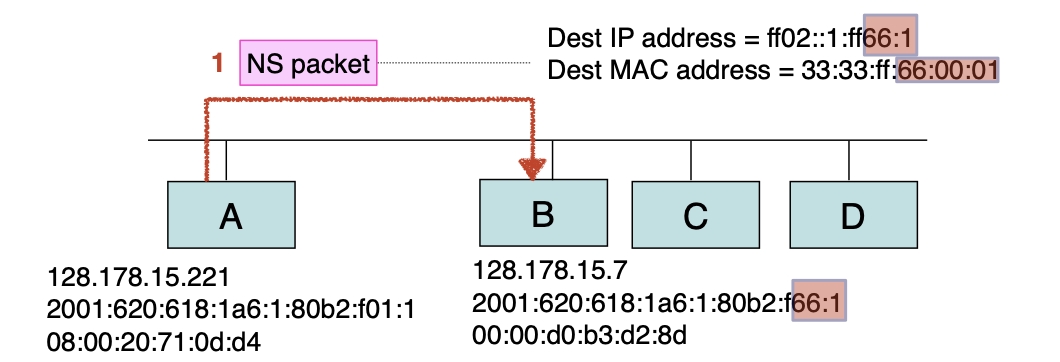
\includegraphics[width=0.7\textwidth]{images/ndp}
    \label{fig:LABEL}
\end{figure}

\underline{Steps:}

i. A sends a \textcolor{blue}{Neighbor Solicitation (NS)} packet with the question: "who has IP address B?"
\begin{itemize}
	\item NS's dest. IP address = a \textcolor{blue}{special multicast address} (Solicited Node Multicast Address) $\Rightarrow$  \textcolor{red}{last 24 bits} are copied by B's IP address
	\item NS's dest. MAC address is derived from the multicast address in a similar way
\end{itemize}


ii. B responds back to A with a \textcolor{blue}{Neighbor Advertisement (NA)} packet, giving its MAC address

iii. A reads B's NA, stores MAC address in its \textcolor{blue}{neighbor cache} (a.k.a \textcolor{blue}{ARP} table) and can send data to B
\begin{itemize}
	\item Cache entries expire after some configurable time of inactivity 
	\item An entry's validity may be extended if positive feedback is received from higher-layer protocols
\end{itemize}

NA, NS packets are carried as \textcolor{red}{ICMPv6} packets

$\Righatrrow$ encapsulated inside IPv6 packets with next-header field = 58 (0x3a)

% Quick centered image
\begin{figure}[H]
    \centering
    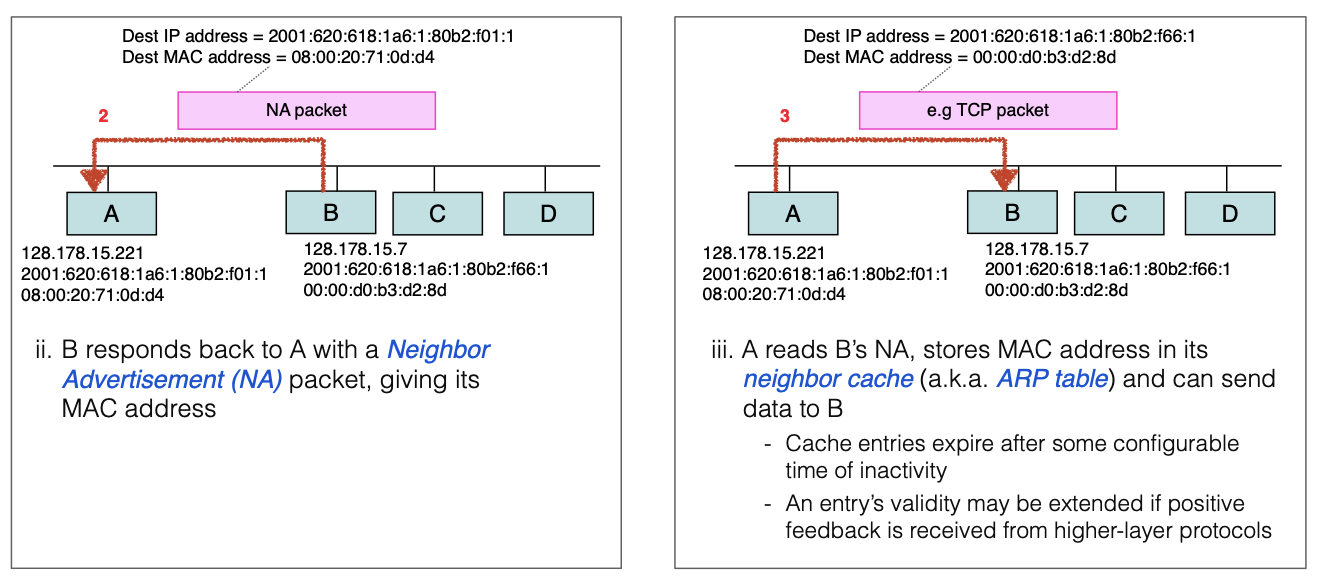
\includegraphics[width=1\textwidth]{images/ndp2}
    \label{fig:LABEL}
\end{figure}


\section*{The Solicited Node Multicast Address in detail}

\begin{itemize}
	\item Obtained by \textcolor{red}{adding last 24 bits} of target IP address to the following \textcolor{red}{prefix: ff02::1:ff00:0/104}
	\item A packet with such a destination address is received by all nodes \textcolor{blue}{all} hosts whose IP address has the \textcolor{blue}{same} last 24 bits (all of them listen/"subscribe" to this multicast address)
	\item Used \textcolor{red}{only} in IPv6 NDP or other protocols; IPv4 uses broadcast instead
\end{itemize}

% Quick centered image
\begin{figure}[H]
    \centering
    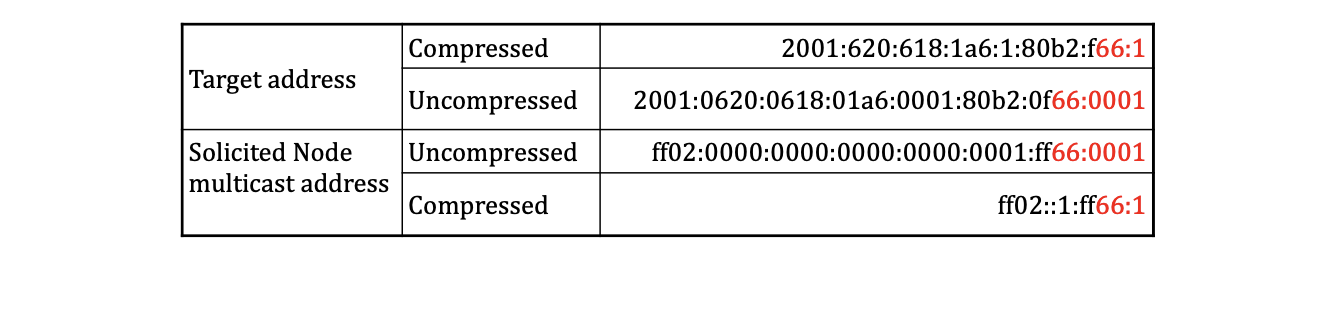
\includegraphics[width=0.9\textwidth]{images/multicast}
    \label{fig:LABEL}
\end{figure}

\section*{Look into an NDP Neighbor Solicitation Packet}

% Quick centered image
\begin{figure}[H]
    \centering
    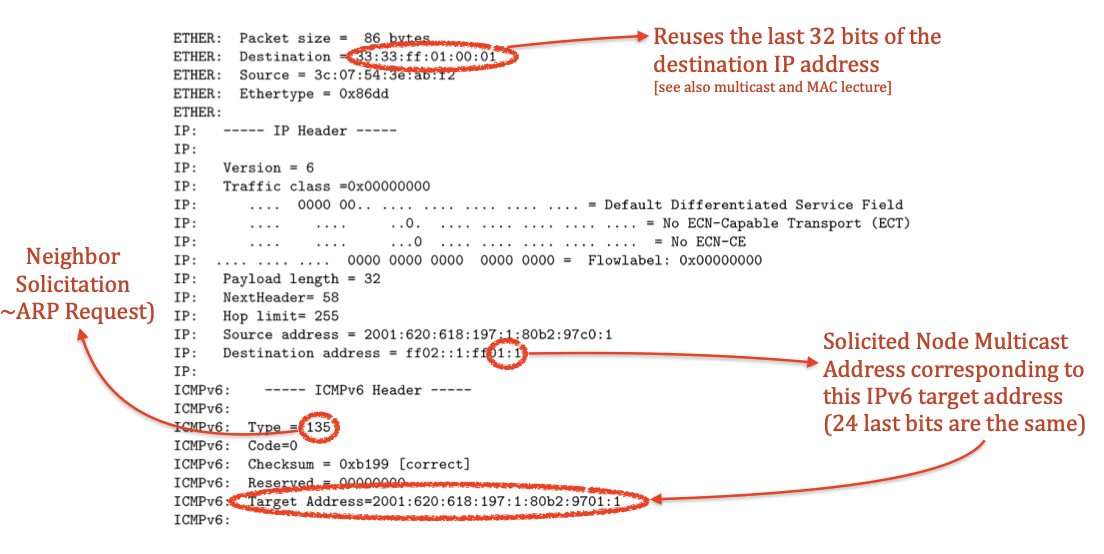
\includegraphics[width=1\textwidth]{images/solicitation-pkt}
    \label{fig:LABEL}
\end{figure}
\section*{MAC Address Resolution with IPv4}

Similar to NDP, except:
\begin{itemize}
	\item Terminology:
		\begin{itemize}
			\item the protocol is called \textcolor{blue}{ARP} (Address Resolution Protocol)
			\item NS/NA pkts of NDP are called \textcolor{blue}{ARP Request/ ARP reply}
		\end{itemize}
	\item Protocol type
		\begin{itemize}
			\item ARP pkts are not ICMP packets (not even encapsulated in IP packets)
		\end{itemize}
	\item Reachability:
		\begin{itemize}
			\item ARP request is \textcolor{red}{broadcast} to all nodes in LAN (instead of multicast)
		\end{itemize}
\end{itemize}

\textbf{Question}: Why don't we do the same like DNS? Having a server that host all the data for MAC resolution address?

\textbf{Solution}: The main reason is that IP address may be reused. If we had a server hosting this information, the server would have to update its entries every time there's changes. 

\section*{Look into an ARP request}
% Quick centered image
\begin{figure}[H]
    \centering
    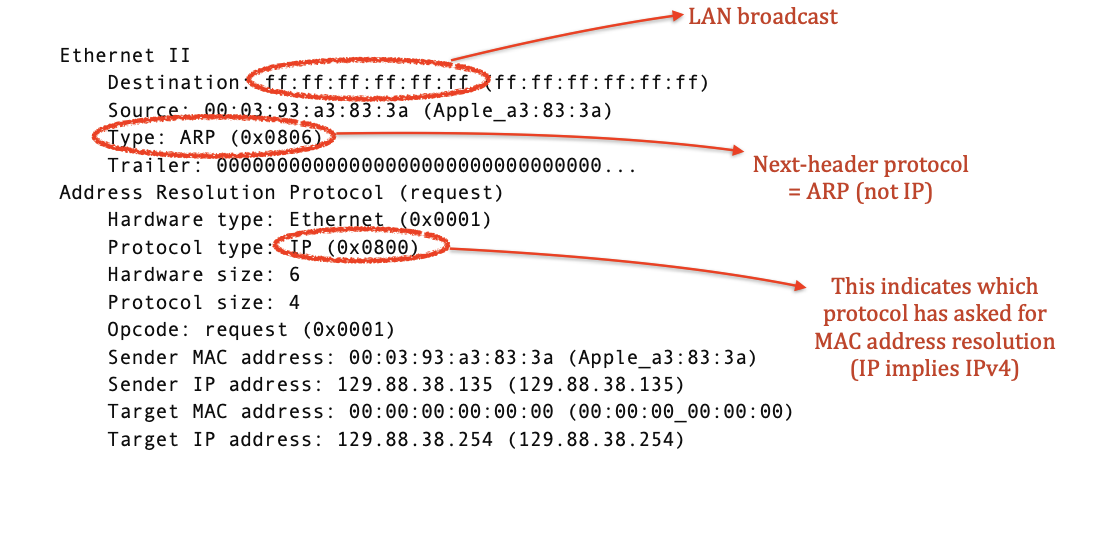
\includegraphics[width=1\textwidth]{images/arp-request}
    \label{fig:LABEL}
\end{figure}

\section*{Security Issues with ARP / NDP}

\begin{itemize}
	\item \textcolor{red}{ARP spoofing}: ARP replies and NAs can be \textcolor{red}{forged}
		\begin{itemize}
			\item attacker intercepts packets destined to B —$>$ easier in IPv4, bc ARP requests are broadcast
	\item sends a bogus NA/ARP reply with its own MAC address
	\item may cause A to map their MAC address to B’s IP address, if the bogus NA arrives \textcolor{blue}{faster} at A
\end{itemize}
\end{itemize}
% Quick centered image
\begin{figure}[H]
    \centering
    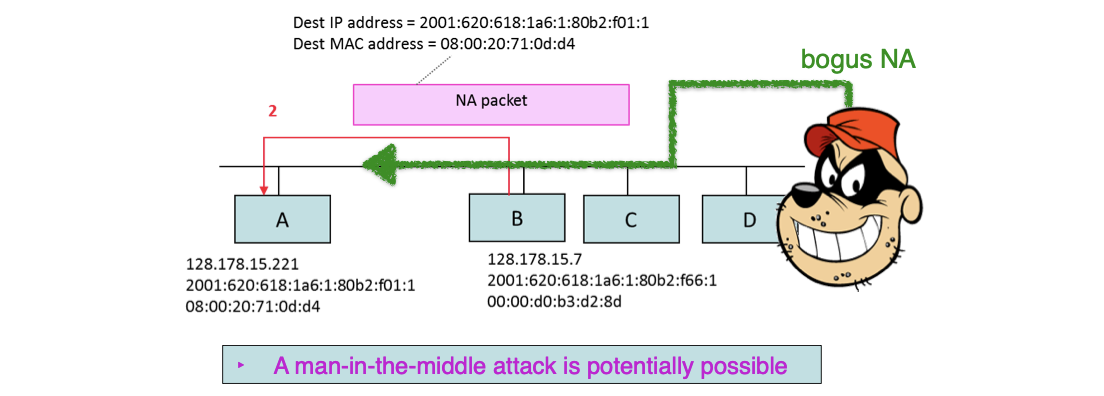
\includegraphics[width=1\textwidth]{images/arp-mitm}
    \label{fig:LABEL}
\end{figure}

\section*{How to prevent ARP spoofing in LANs?}

\begin{itemize}
	\item \textbf{DHCP snooping}: switch/WiFi base station observer all DHCP traffic and remembers mappings IP addr $\Leftrightarrow$ MAC addresses
	\item \textbf{Dynamic ARP inspection}:  switch filters all ARP (or NDP) traffic and allows only valid answers – removes invalid broadcasts (IPv4) and multicasts (IPv6)
	\item Such solutions are deploy in \textcolor{blue}{enterprise networks}, rarely at home or WiFi access points 
\end{itemize}

\vspace{1cm}
\begin{center}
  {\LARGE \textbf{The MAC Layer}}
\end{center}

\vspace{1cm}

\section*{Contents}

1. MAC as Shared Medium \\
2. Switches \\
3. Frame format and MAC addresses \\
4. Virtual LANs \\
5. WiFi Distribution Systems \\
6. Security Aspects \\

\vspace{0.5cm}
\begin{center}
  {\LARGE \textbf{1. MAC: Medium Access Control}}
\end{center}

\vspace{1cm}

The MAC layer is responsible for sharing data between the LAN


\textcolor{red}{Why} invented? So that multiple LAN devices \textcolor{blue}{share} a single physical medium:
\begin{itemize}
	\begin{itemize}
		\item cable (old/coxial Ethernet, Powerline); or
		\item wireless radio link (GSM, WiFI, Bluetooh)
	\end{itemize}
\end{itemize}

\textcolor{red}{What} is the problem?

If several systems transmit at the same time, several frames will appear on the transmission medium (channel) and they will \textcolor{red}{collide/interfere}

Solution 1: joint decoding (allow everyone to talk and decode) -- used in cellular networks (e.g. CDMA)

Solution 2: \textcolor{blue}{mutual exclusion} (only one system can talk at a time), ideally via a \textcolor{blue}{distributed} protocol
\vspace{1cm}

\section*{How to implement mutual exclusion?}

\textcolor{blue}{Deterministic protocols}
\begin{itemize}
	\item use an \textcolor{red}{arbitration} for accessing the transmission medium (channel)
	\begin{itemize}
		\item Time Division Multiple Access (\textbf{TDMA}); each host is given a \textbf{dedicated timeslot} to transmit
	\item Frequency Division Multiple Access (\textbf{FDMA}): each host is given a \textbf{dedicated frequency band} to use
	\item CAN bus: the \textbf{highest-priority} transmitting host dominates other transmission
	\item Token ring, FDDI: every host takes turn and passes a token to next host; whoever has the token, can transmit
		\begin{itemize}
			\item more flexible than TDMA and FDMA, may achieve higher throughput
		\end{itemize}
 	\end{itemize}
	\item \textcolor{red}{avoid} collisions by construction, \textcolor{red}{proactively}
	\item but…work only with few users, as they require synchronization and pre-configuration (if a host goes down or a new one appears, we need to take the network down and reconfigure it)
\end{itemize}

\textcolor{blue}{Stochastic (random access) protocols}
\begin{itemize}
	\item \textcolor{red}{allow everyone} to transmit at any time, \textcolor{red}{detect collisions}, and \textcolor{red}{react}
	\item host transmits at full rate and if a collisions is detected, they retransmit after some \textcolor{blue}{random} time ("\textcolor{blue}{back-off}") 
		\begin{itemize}
			\item WiFi, coaxial/historical Ethernet, Zigbee, signaling channel on cellular networks, Ethernet over Powerline
		\end{itemize}
\end{itemize}

\newpage

\begin{center}
  {\LARGE \textbf{Principles of random-access protocols}}
\end{center}

\vspace{0.5cm}

\section*{ALOHA}

% Quick centered image
\begin{figure}[H]
    \centering
    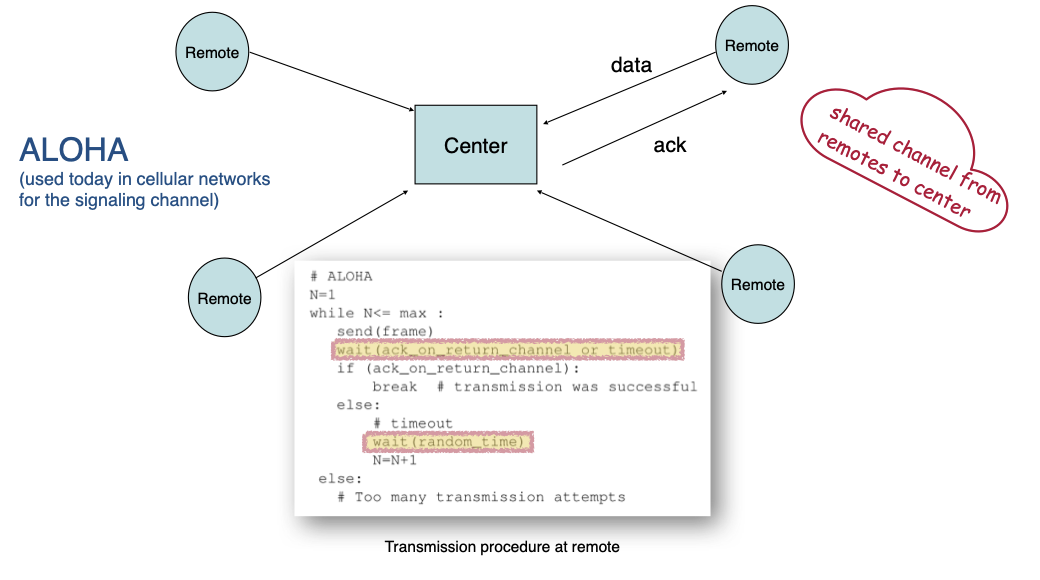
\includegraphics[width=1\textwidth]{images/aloha}
    \label{fig:LABEL}
\end{figure}

\begin{itemize}
	\item Two channels: uplink and downlink. Shared channel from remotes to center. The downlink is easy, the center (radio-station) can schedule it's transmission. 
	\item The others remotes need to schedule their transmission. If they all transmit in the same time, they will collide. 
	\item The \textcolor{blue}{maximum utilization} is \textcolor{red}{18\%} of the channel capacity, which is very small. This is assuming independent and exponential inter-arrival times of pkts and retransmissions.
\end{itemize}

\newpage

\section*{CSMA (carrier sense multiple access)}

\begin{itemize}
	\item Before you transmit, simply listen to the channel. If it's busy, just wait until it's free. It assumes a single \textcolor{blue}{transitive} channel (everyone can hear everyone)
	\item drastically \textcolor{red}{improves efficiency} over Aloha
	\item In CSMA, many collisions can be avoided, but not all. Two or more stations may sense that the medium is idle and start transmitting at time instants that are close enough for a collision to occur (propagation delay is also in the source of this problem)
\end{itemize}

\begin{minipage}{0.5\textwidth}
% Quick centered image
\begin{figure}[H]
    \centering
    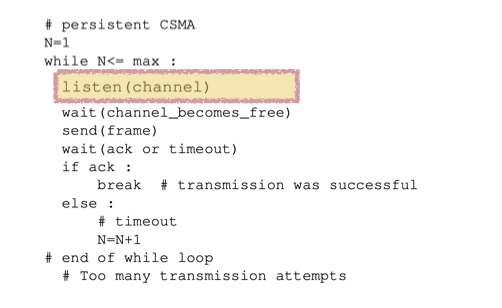
\includegraphics[width=1\textwidth]{images/csma-2}
    \label{fig:LABEL}
\end{figure}
\end{minipage}
\hfill
\begin{minipage}{0.5\textwidth}
\centering
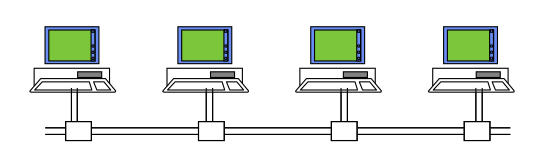
\includegraphics[width=\linewidth]{images/csma}
\end{minipage}

$\Righatrrow$ CSMA works better if: propagation delay is  \textcolor{red}{small}


\section*{Non-persistent CSMA}

\begin{itemize}
	\item uses \textcolor{red}{random} waiting times if channel is busy
	\item avoid hosts' synchronization
		\begin{itemize}
			\item if all stations choose the random delays \textcolor{blue}{independently}, and
	\item if the waiting times are \textcolor{blue}{larger} than the propagation delay
	\item then, with high probability, only one of the transmitting stations seizes the channel
\end{itemize}
	\item improves utilization
\end{itemize}

\newpage

\section*{CSMA / CD (Collision Detection) detects collisions as they occur}

\textcolor{red}{ACKs replaced by CD:} channel is monitored even during transmission to detect collisions
% Quick centered image
\begin{figure}[H]
    \centering
    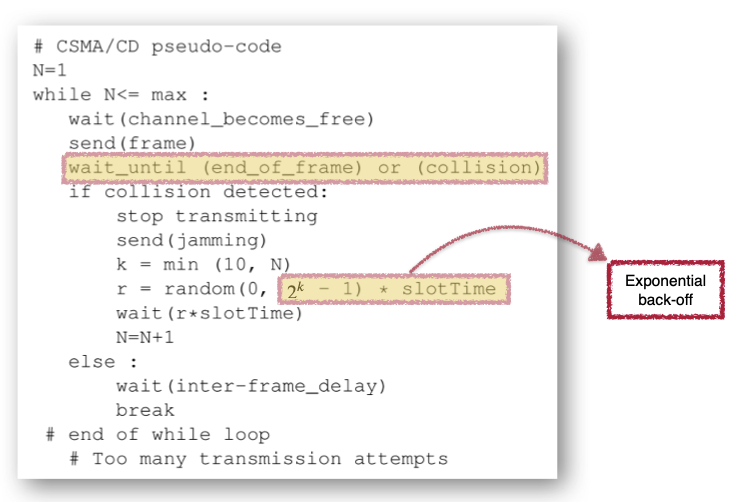
\includegraphics[width=0.8\textwidth]{images/cd}
    \label{fig:LABEL}
\end{figure}

% Quick centered image
\begin{figure}[H]
    \centering
    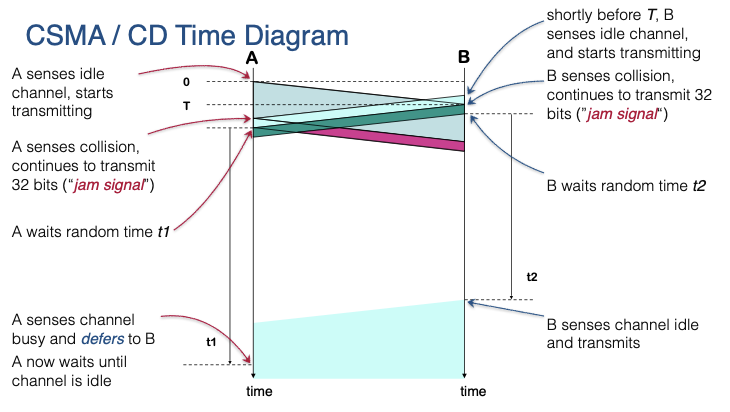
\includegraphics[width=0.8\textwidth]{images/cd-time-diagram}
    \label{fig:LABEL}
\end{figure}
\section*{A Minimum Frame Size is needed to guarantee collision detection}

To avoid undetected collisions, we impose a minimum frame size that depends on the link's \textcolor{red}{bit rate} and round-trip propagation delay \textcolor{red}{(a.k.a slotTime)}

\begin{center}
	transmission delay = frameSize/bitRate $>$ slotTime
$\Rightarrow$ frameSize $>$ slotTime*bitRate $\aprox$ bandwidth-delay product
\end{center}

\section*{CSMA / CD Summary}

\begin{itemize}
	\item CSMA/CD improves on CSMA by requiring that stations detect collisions and stop transmitting (after 32 bits, called \textbf{jam} bits, in order to ensure that all systems properly recognize the presence of collisions).
	\item The jam bits (or jam signal) is a 32-bit binary pattern indicating that a collision has occurred.
	\item CSMA/CD has a \textit{\textcolor{blue}{better performance}} than Aloha or CSMA
	\item After a collision is detected, stations will re-attempt to transmit after a random time
	\item The random time before retransmission is chosen in such a way that if repeated collisions occur, then this time increases exponentially (\textcolor{red}{exponential backoff}). 
	The downside of exponential backoff is that: in case of congestion (too many collisions), the access to the channel is slowed down
	\item Acknowledgements are not necessary because absence of collision means that the frame can be transmitted
	\item An inter-frame delay ("gap") of 9.6$\mu$s is used to avoid blind times, during which adapters are filtering typical noise at transmission ends.
\end{itemize}

\section*{CSMA/CD = early Ethernet (coax cables and hubs)}

Early Ethernet (\textcolor{red}{half-duplex}) addresses \textcolor{blue}{collisions} by using:
\begin{itemize}
	\item CSMA/CD
	\item with restrictions about the slotTime (hence also the min frame size)
		\begin{itemize}
			\item e.g., 10Mbps half-duplex Ethernet uses slotTime = 51.2ms $\Rightarrow$ min frame size = 64Bytes
		\end{itemize}
\end{itemize}

\section*{Wi-Fi = CSMA/CA (Collision Avoidance) = variant of CSMA/CD}

\begin{minipage}{0.6\textwidth}
Uses:
\begin{itemize}
	\item ACKs to detect collisions (i.e. if they are absent)
	\item Carrier sensing, but does not always work:
		\begin{itemize}
			\item e.g., C may be "hidden" from A; 
			\item and this is \textit{mitigated} through \textcolor{blue}{RTS/CTS}
		\end{itemize}
	\item Further optimizations to avoid collisions:
		\begin{itemize}
			\item more \textcolor{red}{conservative channel backoff}. Even if the channel is \verb|idle|, still wait for random time before transmitting
		        \item \textcolor{red}{network allocation vector}. The MAC header contains the transmission time needed for the frame; it its a form of \textcolor{blue}{virtual} carrier sensing
		\end{itemize}
\end{itemize}

\end{minipage}
\hfill
\begin{minipage}{0.4\textwidth}
\centering
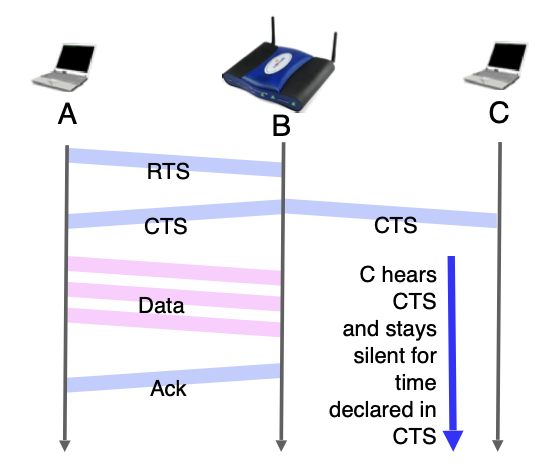
\includegraphics[width=\linewidth]{images/wifi}
\end{minipage}

\begin{tcolorbox}[
  colback=gray!15,     % background color
  colframe=black!50,    % border color
  boxrule=1pt,       % border thickness
  arc=3mm,             % rounded corners
  left=4mm, right=4mm, top=2mm, bottom=2mm % padding
]
\textbf{Question}
In a WiFi network with a single channel and a single
base station, how many data frames can be transmitted
concurrently?

\vspace{0.3cm}

A. At most one in total \\
B. One from mobile to base station and one from base station to mobile \\
C. At most one per mobile to base station and one from base station \\
D. At most one per mobile to base station
and one per mobile from base station \\
E. I don't know \\

\textbf{Solution}: \textcolor{red}{A}. The WiFi MAC layer controls the access of all senders to the radio channel. So, it makes sure that only one can transmit at a time.
\end{tcolorbox}
\end{document}
